\renewcommand{\theequation}{\theenumi}
\begin{enumerate}[label=\arabic*.,ref=\thesubsection.\theenumi]
\numberwithin{equation}{enumi}
\item All the lines can be drawn as follow
\begin{enumerate}
\item put $\vec {x} \myvec{x\\0}$ in equation
\\ 
\begin{align}
\myvec{2 & 3}\myvec{x\\0} &= \frac{187}{20}
\\
x&= \frac{187}{40}
\end{align}
\\
put $\vec {x} \myvec{0\\y}$ in equation
\\
\begin{align}
\myvec{2 & 3}\myvec{0\\y} &= \frac{187}{20}
\\
y&= \frac{187}{60}
\\
\vec{P1} &= \myvec{\frac{187}{40}\\0}
\\\vec{Q1} &= \myvec{0\\\frac{187}{60}}
\end{align}



\item put $\vec{ x} \myvec{x\\0}$ in equation 
\begin{align}
\myvec{1 & -\frac{1}{5}}\myvec{x\\0} &= 10
\\
x&= 10
\end{align}
\\
put $\vec {x} \myvec{0\\y}$ in equation
\\
\begin{align}
\myvec{1 & -\frac{1}{5}}\myvec{0\\y} &= 10
\\
y&= -50
\\
\vec{P2} &= \myvec{10\\0}
\\ \vec{Q2} &= \myvec{0\\-50}
\end{align}


\item put $\vec {x} \myvec{x\\0}$ in equation 
\begin{align}
\myvec{-2 & 3}\myvec{x\\0} &= 6
\\
x&= -3
\end{align}
put $\vec {x} \myvec{0\\y}$ in equation
\\
\begin{align}
\myvec{-2 & 3}\myvec{0\\y}& = 6
\\
y&= 2
\\
\vec{P3} &= \myvec{-3\\0}
\\ \vec{Q3} &= \myvec{0\\2}
\end{align}




\item there is no constant in the line equation thus it passes through the origin.
\\
put $\vec {x} \myvec{3\\y}$ in equation
\\
\begin{align}
\myvec{1 & -3}\myvec{3\\y} &= 0
\\
y&= 1
\\
\vec{P4} &= \myvec{0\\0}
\\ \vec{Q4} &= \myvec{3\\1}
\end{align}


\item there is no constant in the line equation thus it passes through the origin
\\
put $\vec {x} \myvec{1\\y}$ in equation
\\
\begin{align}
\myvec{2 & -1}\myvec{1\\y} &= 0
\\
y&= 1
\\
\vec{P5}& = \myvec{0\\0}
\\ \vec{Q5} &= \myvec{1\\2}
\end{align}


\item put $\vec {x} \myvec{x\\0}$ in equation
\begin{align}
\myvec{3 & 0}\myvec{x\\0}&= -2
\\
x&= -\frac{2}{3}
\end{align}
\\
we can see in this equation the  value of x coordinate does not depend on the y coordinate so we can say that it is parallel to the y-axis.





\item put $\vec {x} \myvec{x\\0}$ in equation 
\begin{align}
\myvec{0& 1}\myvec{0\\y} &= 2
\\
y&= 2
\end{align}
\\
we can see in this equation the  value of y coordinate does not depend on the x coordinate so we can say that it is parallel to the x-axis.



\item put $\vec {x} \myvec{x\\0}$ in equation 
\begin{align}
\myvec{2 & 0}\myvec{x\\0} &= 5
\\
x&= -\frac{5}{2}
\end{align}
\\
we can see in this equation the  value of x coordinate does not depend on the y coordinate so we can say that it is parallel to the y-axis.
\begin{figure}[!ht]
	\centering
	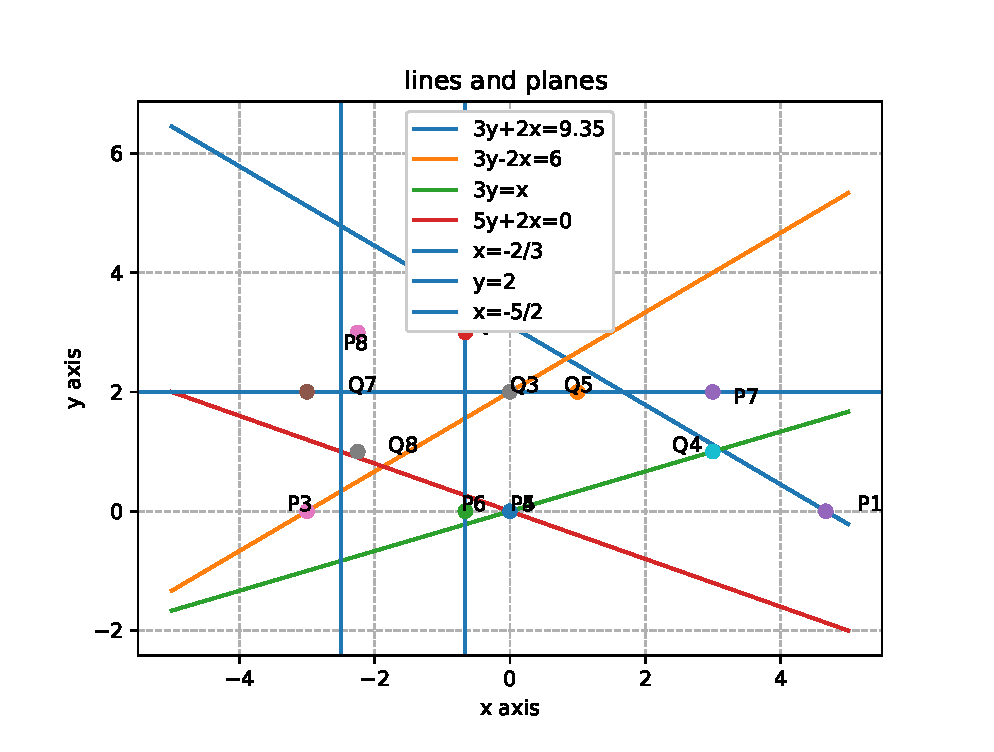
\includegraphics[width=\columnwidth]{./figures/line/lines_and_planes/lines_and_planes.eps}
	\caption{lines }
	\label{fig:lines}
	Path to the python code for the above figure
	\begin{lstlisting}
	codes/line/lines_and_planes/plane_and_line.py
	\end{lstlisting} 
\end{figure}

\end{enumerate}
\end{enumerate}